\chapter{Magic}\label{chap:magic}

\begin{figure}[!htb]
\centering
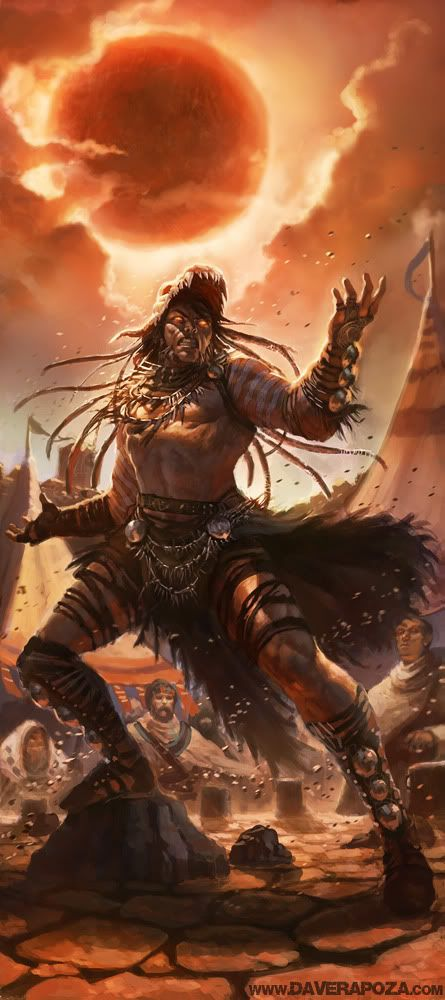
\includegraphics[width=0.3\linewidth]{images/defiler.jpg}
\end{figure}

\epigraph{\textit{
    "The Tablelands are a giant wasteland, to the untrained eye barren and devoid of life. When people see plants wither and
    die when someone utters mysterious phrases accompanied by unknown gestures, they assume the worst. They cry wizard
    and the mob instantly gathers to kill him. But if people venture into the wastes and look under the rocks, they will learn
    that Athas is teeming with all sorts of life. And when the vermin swarm forth to envelop them, biting and crawling into
    every orifice, do they see the irony?" } } { The Oracle, Blue Shrine Scrolls }


\begin{table*}[!htb]
\begin{GenesysTable}{Penalties when casting spells}{casting-penalties}{ =X +l}
Condition                                                       & Penalty\\
The character does not have a free hand                         & +\setback \\
The character is gagged, silenced or otherwise unable to speak  & +\setback\setback \\
Penalty per 1 encumbrance of armor above 1                      & +\setback \\
The character is in circumstances that interfere
with their ability to concentrate, such as trying
to cast while swimming or hanging from a rope,
being buffeted by a sandstorm, or casting a spell
that doesn't target the person they're fighting in
hand-to-hand combat.                                           & +1 or more \difficulty \\
\end{GenesysTable}
\end{table*}

\begin{table*}[!htb]
\begin{GenesysTable}{Spending Threat and Despair when casting spells}{casting-spending-threat}{ =l +X}
Cost                                &   Result\\
\threat or \despair                 &   The magical energies exhaust the player, they suffer 2 strain or 1 wound (GM's choice)\newline
                                        \newline
                                        (When using the Defiling action) Plantlife in the area turns to ash. Using more \threat or \despair upgrades the area, or even includes wildlife.\newline
                                        \newline
                                        All arcane and primal casters, including the caster, suffer \setback untill this players next turn.\\
\threat\threat or \despair          &   The spell doesn’t take effect until the start of the next round, or after a minute in narrative gameplay.\newline
                                        \newline
                                        Until the end of the encounter, enemy spellcasters add \boost when casting a spell that targets this character.\\
\threat\threat\threat or \despair   &   The spell is slightly more powerful than expected. One character of the GM's choice is targeted or otherwise affected by the spell as well.\newline
                                        \newline
                                        All other spellcasters and creatures attuned to magical energies within a day's travel become aware of the character (and depending on
                                        their disposition, may be very interested in finding them and doing them harm). \\
\despair                            &   The character overexerts themself or loses their magical connection and is unable to cast spells for the rest of the encounter or scene.\newline
                                        \newline
                                        The Spell Component used is exhausted and cannot be used anymore this scene. If it is an Arcane Spell Components, it is also damaged.\newline
                                        \newline
                                        The GM picks the target of the character's spell. If the caster is an NPC, the controlling player picks the target of the spell instead.\\
\despair\despair                    &   The character completely lose control of their magical energies or draws the ire of their deity, suffering one Critical Injury (at the GM's
                                        discretion, this may instead take the form of some of terrible or hilarious misfortune, such as temporarily being turned into a small woodland
                                        creature, being struck by lightning on a clear day, swapping bodies with someone else in the encounter for the remainder of the day, or
                                        summoning an avatar of elemental wrath).\newline
                                        \newline
                                        (When using the Defiling action) A ally of the player gains a number of wounds equal to the number of \threat rolled.\newline
                                        \newline
                                        If the caster is using an Arcane Spell Component, the component has lost it's magical potential and is destroyed.\\
\end{GenesysTable}
\end{table*}

\FloatBarrier

\begin{multicols}{2}

\section{Magical Manouvers}
To use these manouvers, the character has to have atleast 1 rank in either
an Arcane or an Primal skills and have a talent allowing them to use that
skill to cast spells.

\subsection{Counterspell}
Most skilled mages or spellcasters can attempt to counter an opponent’s spells
as they are being cast. If the character performs the counterspell maneuver,
all opponents within medium range upgrade the difficulty of checks to cast
spells once, until the end of the character's next turn.

\subsection{Concentrate}
Some magical effects might require concentration to sustain. If a magical action
(or spell) can benefit from concentration, the action description notes this.
Spells that can be sustained through concentration last until the end of the
character's next turn (as noted in their description). However, if the character
performs the concentrate maneuver during that next turn, the spell’s effects last
until the end of the character’s following turn, instead. This can be sustained
indefinitely by performing the concentrate maneuver each turn.

\section{Arcane}
Characters can only use one of the Arcane skills to cast a spell if they have a talent
allowing such use. Each spell has various options to raise the overal difficulty
of the check, in exchange for various benefits. The overal difficulty of
such a check can never be raised beyond (\difficulty\difficulty\difficulty\difficulty\difficulty),
after reductions. Casting a spell costs 2 Strain. In addition, when casting an
arcane spell the user adds a number of \force die equal to the ranks of the skill
used in the spell. Any one \darklight thrown during the skill check can be used to
substitute a \advantage, and \darklight\darklight\darklight can be used to substitute
a \success.\\
However, using \light cost an extra Strain, simulating the extra energy used from
within and \dark used during casting constitude the use of Defiling magic. The GM
is encouraged to narrate this effect on the environment and it is certainly possible
that there are actual consequences for its use, with more \darklight constituting
greater defilement. People will notice defiling magic, especially when it is used
often or a lot \darklight is used at once.

Finally Arcane magic can use Spell Components to enhance the potenty of their spells
or reduce their difficulty. (See \cref{itmmgc:spellcomponentpouch} for more information).

\paragraph{Preserving}
\textbf{Preserving} is when an arcane spell is cast without using any \dark, regardless of the number of \light used.
Talents requiring preserving can thus be only used when the caster does not use any \dark in the casting of that spell.

\paragraph{Defiling}
\textbf{Defiling} is when an arcane spell is cast using atleast one \dark, regardless of the number of \light used.
Talents requiring defiling can thus only be used when the caster uses atleast any \dark.

\end{multicols}

\hrulefill

\begin{multicols}{2}
\subsection{Arcane Spells}
\begin{table*}[!htb]
\begin{GenesysTable}{Attack Additional Effects}{magic-attack}{ =l +X}
Cost                    & Effect\\
\difficulty             & \textbf{Blast:} The attack gains the \iqtyref{blast} quality with a rating equal to your character's ranks in Attack.\\
\difficulty             & \textbf{Close Combat:} May select a target engaged with your character.\\
\difficulty             & \textbf{Deadly:} The attack gains a Critical rating of 2. The attack also gains the \iqtyref{vicious} quality with a rating
                            equal to the character's in knowledge\\
\difficulty             & \textbf{Fire:} The attack gains the \iqtyref{burn} quality with a rating equal to your character's ranks in Attack.\\
\difficulty             & \textbf{Impact:} The attack gains the \iqtyref{knockdown} quality. The attack also gains the Disorient quality with a
                            rating equal to the character's ranks in Attack.\\
\difficulty             & \textbf{Lightning:} The attack gains the \iqtyref{stun} quality with a rating equal to the character's ranks in Attack.
                            The attack also gains the \iqtyref{autofire} quality. (You must increase the difficulty by one to use the
                            Auto-fire quality as normal.)\\
\difficulty             & \textbf{Manipulative:} If the attack hits, you may spend \advantage to move the target up to one
                            range band in any direction.\\
\difficulty             & \textbf{Non-Lethal:} The attack gains the \iqtyref{stundamage} quality.\\
\difficulty             & \textbf{Range:} Increase the range of the spell by one range band. This may be added multiple times, increasing
                            the range by one range band each time.\\
\difficulty             & \textbf{Quick Sand:} The attack gains the \iqtyref{ensnare} quality with a rating equal to the character's ranks in Attack.\\
\difficulty\difficulty  & \textbf{Destructive:} The attack gains the \iqtyref{sunder} quality. The attack also gains the Pierce quality with a
                            rating equal to the character's ranks in Attack.\\
\difficulty\difficulty  & \textbf{Empowered:} The attack deals damage equal to twice the characteristic linked to the skill (instead
                            of dealing damage equal to the characteristic). If the attack has the \iqtyref{blast} quality, it affects
                            all characters within short range, instead of engaged.\\
\difficulty\difficulty  & \textbf{Poisonous:} If the attack deals damage, the target must immediately make a
                            Hard(\difficulty\difficulty\difficulty) Resilience check or suffer wounds equal to the character's
                            ranks in Attack, and strain equal to the character's ranks in Attack. This counts as a poison.\\
\end{GenesysTable}
\end{table*}

\subsubsection{Attack}
\fxnote{\currentname: Check and perhaps rephrase this.}
\textbf{Skill:} Arcane Attack\\
\textbf{Concentration:} No\\
\textbf{Basic Difficulty:} \textbf{Easy:} (\difficulty)\\
Magic attacks are cast spell checks but additionally follow the normal rules for
performing combat checks. When making a magic attack the character must select
one target at short (but not enganged) range. The attack deals damage equal to
the casters Intellect plus one per uncancelled \success. The attack has no
critical rating, so you may only inflict a Critical Injury with a \triumph.
Before making a magical attack, you may choose any number of additional effects
from~\tableref{magic-attack}.


\begin{table*}[!htb]
\begin{GenesysTable}{Barrier Additional Effects}{magic-barrier}{ =l +X}
Cost                    & Effect\\
\difficulty             & \textbf{Additional Target:} The spell affects one additional
                            target within range of the spell. In addition, after
                            casting the spell, you may spend \advantage to affect
                            one additional target within range of the spell (and
                            may trigger this multiple times, spending \advantage
                            each time).\\
\difficulty             & \textbf{Range:} Increase the range of the spell by one range band.
                            This may be added multiple times, increasing the range
                            by one range band each time.\\
\difficulty\difficulty  & \textbf{Add Defense:} Each affected target gains ranged and melee
                            defense equal to your ranks in Barrier.\\
\difficulty\difficulty  & \textbf{Empowered:} The barrier reduces damage equal to the
                            number of uncanceled \success instead of the normal
                            effect.\\
\end{GenesysTable}
\end{table*}

\subsubsection{Barrier}
\fxnote{\currentname: Check and perhaps rephrase this.}
\textbf{Skill:} Arcane Barrier\\
\textbf{Concentration:} Yes\\
\textbf{Basic Difficulty:} \textbf{Easy:} (\difficulty)\\
Both arcane and divine spellcasters have the power to
create barriers of magical energy to protect themselves
and their allies. The character selects one target they are
engaged with (which can be themself), then makes an
Arcana or Divine skill check.  If the check is successful,
until the end of the character’s next turn, reduce the damage
of all hits the target suffers by one, and further reduce it
by one for every uncanceled \success\success beyond the first.
Before making an Barrier check, you may choose any number of
additional effects from ~\tableref{magic-barrier}.


\begin{table*}[!htb]
\centering
\small\caption{Dispel Additional effects}
\begin{GenesysTable}{l X}
Cost                    & Effect\\
\difficulty             & \textbf{Range:} Increase the range of the spell by one range band. This may be added multiple times, increasing the range by one range band each time.\\
\difficulty\difficulty  & \textbf{Additional Target:} The spell affects one additional target within range of the spell. In addition, after casting the spell, you may
                            spend \advantage to affect one additional target within range of the spell (and may trigger this multiple times, spending \advantage each time).\\
\end{GenesysTable}
\label{table:magic_dispel}
\end{table*}

\subsubsection{Dispel}
\textbf{Skill:} Arcane\\
\textbf{Concentration:} No\\
The ability to nullify magic is a strange and wondrous
art that only certain arcane spellcasters possess. The
character selects one target within short range that
is under the effects of a spell, then makes an Arcana
 skill check. The default difficulty for the check is Hard
(\difficulty\difficulty\difficulty). If the check is successful,
the effects the target is under immediately end (if the spell
affected multiple targets, the other targets remain affected).
Before making a dispel check, choose any number of additional
effects from ~\tref{table:magic_dispel}.


\begin{table*}[!htb]
\begin{GenesysTable}{Enchantment Additional Effects}{magic-enchantment}{ =l +X}
Cost                    & Effect\\
\difficulty             & \textbf{Influence Emotions:} The target is filled with an
                            overwhelming amount of a specific emotion of the
                            caster's choice, such as anger, calm, disgust, fear,
                            friendliness, or peace. The caster learns the Strength
                            or Flaw of the targeted character.\\
\difficulty             & \textbf{Additional Target:} The spell affects one additional
                            targets within range of the spell. In addition,
                            after casting the spell, you may spend \advantage to affect
                            one additional target within range of the spell (and
                            may trigger this multiple times, spending \advantage each time).\\
\difficulty             & \textbf{Compulsion:} The spell targets any one non-nemesis target,
                            and if successful, it is forced to believe something
                            untrue or assist the Spellcaster and their allies on
                            a task for one turn or five minutes. The target is
                            aware of all its actions and will not perform any action
                            that might harm it or its direct allies. In addition,
                            after casting the spell, you may spend \advantage\advantage
                            to increase the length of the effect by one additional
                            turn or five more minutes.\\
\difficulty             & \textbf{Duration:} The \advantage bonus applies to the next two checks
                            the caster makes. In addition, after casting the spell,
                            you may spend \advantage to apply the bonus to the third
                            check the caster makes (and may trigger this multiple
                            times, spending \advantage each time).\\
\difficulty\difficulty  & \textbf{Modify Memory:} The target completely forgets the last
                            five minutes of its conscious existence. In addition,
                            after casting the spell, you may spend \advantage to
                            increase the length of time forgotten by an additional
                            five minutes, (and may trigger this multiple times,
                            spending \advantage each time).\\
\difficulty\difficulty  & \textbf{Strength:} The caster adds \success equal to \success,
                            and \advantage equal to \advantage to their social
                            skill check.\\
\difficulty\difficulty  & \textbf{Dominate:} The target obeys all commands given to it by
                            the caster for one round or for five minutes. In
                            addition, after casting the spell, you may spend \advantage
                            to increase the length of time forgotten by an
                            additional five minutes, (and may trigger this
                            multiple times, spending \advantage each time).\\
\end{GenesysTable}
\end{table*}

\subsubsection{Enchantment}
\textbf{Skill:} Arcane\\
\textbf{Concentration:} Yes\\
\textbf{Basic Difficulty:} \textbf{Average:} (\difficulty\difficulty)\\
By practicing the art of Enchantment spellcasters lace their words with magic,
allowing them to compel, terrify, and beguile their targets. A character selects
one target they are engaged with the makes an Arcana check. If the check is
successful, the caster adds a equal to \advantage to their next social skill
check against the target. Before making an Enchantment check, you may choose
any number of additional effects from ~\tableref{magic-enchantment}.

\begin{table*}[!htb]
\begin{GenesysTable}{Illusion Additional Effects}{magic-illusion}{ =l +X}
Cost                                & Effect\\
\difficulty                         & \textbf{Additional Illusion:} The spell creates an
                                        additional visual illusion. You may spend
                                        \advantage\advantage to create one additional
                                        visual illusion.\\
\difficulty                         & \textbf{Additional Target:} The spell affects three
                                        additional targets within range of the spell.
                                        In addition, after casting the spell, you may
                                        spend \advantage to affect two additional
                                        targets within range of the spell (and may
                                        trigger this multiple times, spending
                                        \advantage each time).\\
\difficulty                         & \textbf{Conceal:} Until the beginning of the user's turn,
                                        the target cannot see or sense a chosen
                                        person or object of silhouette 1 or smaller.
                                        The chosen person or object must remain
                                        stationary or the spell fails.\\
\difficulty                         & \textbf{Increased Size:} The spell creates an illusion
                                        up to silhouette 3 or conceals a static
                                        object up to silhouette 2.\\
\difficulty                         & \textbf{Movement:} The spell creates an illusion with
                                        basic movements and gestures, and can patrol
                                        in an area of up to short range. You may
                                        spend \advantage\advantage to increase the
                                        range the illusion can move by one range band
                                        per \advantage\advantage.\\
\difficulty                         & \textbf{Range:} Increase the range of the spell (the
                                        distance from the character the illusion
                                        effect appears) by one range band. You may
                                        spend \advantage\advantage to extend the
                                        range band by one (and may trigger this
                                        multiple times, spending \advantage\advantage
                                        each time).\\
\difficulty                         & \textbf{Simultaneous Effect:} The spell creates one
                                        additional sensory effect that appears in
                                        sync with the visual component of the illusion.
                                        You may spend \advantage\advantage to create
                                        one additional visual or sensory effect.\\
\difficulty                         & \textbf{Silence:} The spell causes all sound within an
                                        area of 20 feet to be inaudible to any
                                        creature outside the area.\\
\difficulty\difficulty              & \textbf{Disguise:} The spell alters the target's
                                        entire appearance, either physically or
                                        by adding/subtracting clothing, gear,
                                        personal effects, or other. You may spend
                                        \advantage\advantage to alter how the target
                                        sounds or smells. Nothing this spell creates
                                        has a physical component, so objects pass
                                        through it as normal, and any creature that
                                        touches it will feel nothing.\\
\difficulty\difficulty              & \textbf{Massive Size:} The spell creates an illusion up
                                        to silhouette 4.\\
\difficulty\difficulty\difficulty   & \textbf{Invisibility:} The target is invisible and gains
                                        \triumph on any Stealth checks it makes for
                                        as long as concentration is maintained. You
                                        may spend \advantage\advantage to render all
                                        sounds the target makes inaudible.\\
\end{GenesysTable}
\end{table*}

\subsubsection{Illusion}
\textbf{Skill:} Arcane\\
\textbf{Concentration:} Yes\\
\textbf{Basic Difficulty:} \textbf{Easy:} (\difficulty)\\
Arcane spellcasters can influence the mind of a target, causing
it to see, hear, or smell something that is not there. Likewise, they can cause
the target to not see, hear, or smell something.  The characters selects up to
three targets in short range, then makes either an Arcana or Divine skill check.
If the check is successful, the targets either sees a single static image up to
a size of silhouette 2, hears a sound ranging from a whisper to a scream emanating
from close range, or smells something wafting from close range. Likewise, the spell
can cause the target to be unable to see a small, static object with silhouette 1
such as a chest, weapon, door, or shelf. Before making an Illusion check, choose
any number of additional effects from ~\tableref{magic-illusion}.

\subsubsection{Cantrip}
\textbf{Skill:} Any Arcane\\
\textbf{Concentration:} Yes\\
\textbf{Difficulty:} \textbf{Easy:} (\difficulty)\\
Cantrips covers all the minor things that we expect
people to be able to do with magic, such as levitating a
book, transmuting a pebble into a butterfly, detecting
something magical nearby, summoning a ghostly light
source to see in the dark, or making one’s voice growl
with distant thunder. Basically, these are all cool abilities
with a minor benefit, but are more tricks than dangerous
or powerful magics. That doesn’t mean a player can't fig-
ure out how their character can use a utility spell to their
best advantage—that’s half the fun of being a spellcaster!

Cantrips don't have an equivalent action for
structured encounters, since the effects are almost
entirely narrative in nature. A check to cast a utility spell
should always be Easy (\difficulty). If that check seems too easy
for what you want to accomplish, then what you want to
do is probably beyond the scope of the cantrips!


\end{multicols}

\FloatBarrier
\hrulefill

\begin{multicols}{2}

\section{Primal}

As with Arcana, Characters can only use one of the Primal skills to cast a spell if they
have a talent allowing such use. Each spell has various options to raise the overal
difficulty and the use of Primal Spell Components can be used to enhance the potenty
of their spells or reduce their difficulty. (See \cref{itmmgc:spellcomponentpouch}
for more information). Primal Castes do not use \force dice.

\subsection{Primal Spells}
\begin{table*}[!htb]
\centering
\small\caption{Augment Additional Effects}
\begin{GenesysTable}{l X}
Cost                    & Effect\\
\difficulty             & \textbf{Haste:} Targets affected by the spell can always perform
                            a second maneuver during their turn without spending
                            strain (they may still only perform two maneuvers a turn).\\
\difficulty             & \textbf{Fury:} The target adds damage equal to the character's
                            ranks in Knowledge to unarmed combat checks, and their
                            Critical rating for unarmed combat checks becomes 3.\\
\difficulty             & \textbf{Range:} Increase the range of the spell by one range band.
                            This may be added multiple times, increasing the range
                            by one range band each time.\\
\difficulty             & \textbf{Swift:} Targets affected by the spell ignore the effects
                            of difficult terrain and cannot be immobilized.\\
\difficulty\difficulty  & \textbf{Additional Target:} The spell affects one additional target
                            within range of the spell. In addition, after casting
                            the spell, you may spend \advantage to affect one
                            additional target within range of the spell (and may
                            trigger this multiple times, spending \advantage each time).\\
\end{GenesysTable}
\label{table:magic_augment}
\end{table*}

%TODO: rephrease text
%TODO: replace Knowledge
\subsubsection{Augment}
\textbf{Skill:} Primal\\
\textbf{Concentration:} Yes\\
\textbf{Basic Difficulty:} \textbf{Average:} (\difficulty\difficulty)\\
This is using magic to enhance people. A character selects
one target they are engaged with (which can be themself),
then makes a Primal skill check. If the check is successful,
until the end of your character's next turn, the target
increases the ability of any skill checks they make by one
(in effect, this means they add \proficiency to their checks).
A character may not be affected by more than one Augment spell
at the same time (so no stacking effects).
Before making an augment check, you may choose any number of
additional effects from ~\tref{table:magic_augment}.

\begin{table*}[!htb]
\centering
\small\caption{Conjure Additional Effects}
\begin{GenesysTable}{l X}
Cost                    & Effect\\
\difficulty             & \textbf{Additional Summon:} The spell summons one additional
                            item, weapon, or creature. In addition, after casting
                            the spell, you may spend \advantage\advantage to
                            summon one additional item, weapon, or creature (and
                            may trigger this multiple times, spending
                            \advantage\advantage each time).\\
\difficulty             & \textbf{Medium Summon:} The character may summon a more
                            complicated tool with moving parts, a rival no larger
                            than silhouette 1, or a two-handed melee weapon.\\
\difficulty             & \textbf{Range:} Increase the range of the spell (the distance
                            from the character that the summoned item or creature
                            appears) by one range band. This may be added multiple
                            times, increasing the range by one range band each time.\\
\difficulty             & \textbf{Summon Ally:} The creature the character summons is
                            friendly to them and obeys their commands. The character
                            may spend a maneuver to direct the creature, allowing
                            them to determine its action and maneuver. (If the
                            character summons multiple creatures, the character
                            may spend one maneuver on their turn to direct the
                            turns of all summoned creatures.)\\
\difficulty\difficulty  & \textbf{Grand Summon:} The character may summon a rival of up to
                            silhouette 3.\\
\end{GenesysTable}
\label{table:magic_conjure}
\end{table*}

%TODO: rephrease text
\subsubsection{Conjure}
\textbf{Skill:} Primal\\
\textbf{Concentration:} Yes\\
\textbf{Basic Difficulty:} \textbf{Easy:} (\difficulty)\\
This action represents the ability of a spellcaster to animate objects or create
items (or even allies) out of thin air and the aether. The character makes a Primal
skill check. If the check is successful, the character summons a simple tool with
no moving parts (such as a shovel or pickax), a one-handed melee weapon with no moving
parts (such as a sword or knife), or a minion no bigger than silhouette 1 (such as an
animal, magical creature, elemental spirit, or even undead monstrosity). These appear
engaged with the character. The summoned minion or item remains present until the end
of the character's next turn. If the character summons a creature, the creature behaves
in the best approximation of its natural instincts (as determined by the GM). It
is not controlled by the character, and may even be hostile to them. In a structured
encounter, it takes its turn immediately after the character. Before making an
Conjure check, you may choose any number of additional effects from
~\tref{table:magic_conjure}.


\begin{table*}[!htb]
\centering
\small\caption{Curse Additional Effects}
\begin{GenesysTable}{l X}
Cost                               & Effect\\
\difficulty                        & \textbf{Enervate:} If a target suffers strain for any
                                        reason, they suffer 1 additional strain.\\
\difficulty                        & \textbf{Misfortune:} After the target makes a check,
                                        you may change one \boost to a face displaying a \threat.\\
\difficulty                        & \textbf{Range:} Increase the range of the spell by one
                                        range band. This may be added multiple times,
                                        increasing the range by one range band each time.\\
\difficulty\difficulty             & \textbf{Additional Target:} The spell affects one
                                        additional target within range of the
                                        spell. In addition, after casting the
                                        spell, you may spend \advantage to affect
                                        one additional target within range of the
                                        spell (and may trigger this multiple times,
                                        spending \advantage each time).\\
\difficulty\difficulty             & \textbf{Despair:} The target's strain and wound thresholds
                                        are reduced by an amount equal to the
                                        character’s ranks in Knowledge. This effect
                                        may not be combined with the additional
                                        target effect.\\
\difficulty\difficulty             & \textbf{Doom:} After a target makes a check, you may
                                        change any one die in the pool not displaying
                                        a \failure or \triumph to a different face.\\
\difficulty\difficulty\difficulty  & \textbf{Paralyzed:} The target is staggered for the
                                        duration of the spell. This affect may not
                                        be combined with the additional target effect.\\
\end{GenesysTable}
\label{table:magic_curse}
\end{table*}

%TODO: rephrease text
%TODO: replace Knowledge
%TODO: check dice faces
\subsubsection{Curse}
\textbf{Skill:} Primal\\
\textbf{Concentration:} Yes\\
This action represents the combat use of curse magic. Your
character selects one target within short range, then makes
an Arcana or Divine skill check. The default difficulty of
the check is Average (\difficulty\difficulty). If it is successful, until the
end of the character’s next turn, the target decreases the
ability of any skill checks they make by one (in effect, this
means they remove one \proficiency from their checks).
 
Before making an Curse check, you may choose any number of
additional effects from ~\tref{table:magic_curse}.

\begin{table*}[!htb]
\centering
\small\caption{Shape Additional Effects}
\begin{GenesysTable}{l X}
Cost                                & Effect\\
\difficulty                         & \textbf{Entangle:} All creatures in the affected area are Immobilized.\\
\difficulty                         & \textbf{Range:} Increases the range of the spell by one range band.\\
\difficulty                         & \textbf{Radius:} The size of the area increases by one range band. This may be added again to further increase the size.\\
\difficulty                         & \textbf{Precision:} The character may select one creature within the area to remain unaffected. You may spend one \advantage to select an additional creature.\\
\difficulty\difficulty              & \textbf{Burn:}  All creatures in the area suffer \nameref{iqty:burn} damage equal to the character's ranks in the Knowledge skill.\\
\difficulty\difficulty\difficulty   & \textbf{Quick Sand:} All characters in the area are Paralysed and immune to all damage. The area is impassable terrain. This cannot be combined with Precision.\\
\end{GenesysTable}
\label{table:magic_shape}
\end{table*}

\subsubsection{Shape}
\textbf{Skill:} Arcane\\
\textbf{Concentration:} Yes\\
Shape spells change the area around them. A druid compels the plants to grow into
aggressive, grasping vines to entangle anything that moves. A wizard creates a
sheets of slippery, flammable grease in the path of her gith persuers.
Pooling their power together, a group of cultists call forth a swirling storm of
spirits that rip at the armor of the adventuring party that seeks to stop them.\\

Shaping magic is how spellcasters exert their will over an entire battlefield.
Though it does little against a single adversary compared to other magic, shapping
magic can effect a wide area for an extended period, completely changing the course
of an encounter. Shaping magic generally does no damage - instead, it restricts
movement. In its most basic form, it turns an area into difficult terrain. As a
rule, shaping magic does not exclude the caster or their allies. All characters
within the affected area suffer its effects unless the caster increases the
difficulty. The caster selects a point within medium range, and everything within
short range of that point is affected.\\

The default difficulty of the check is Average (\difficulty\difficulty).
At higher levels a shape spell may immobilize creatures, create an area of total
silence, or simply freeze everything inside a huge block of salt.\\
Before making an Shape check, choose any number of additional
effects from ~\tref{table:magic_shape}.


\FloatBarrier

\section{Psionics}
Your rank in the Psionics skill determines your psionics rating.
When using a psionics power, you roll a number of \force die equal to your
psionics rating. You can use \darklight to enhance your psionics power,
using \light is free, however \dark points show that you have a harder time,
if you want to use \dark points, you lose 1 Strain for each \dark point you
use.\\
\\
In contrast to the Arcana and Primal skills, anyone with one or more ranks
in Psionics can buy and use a Psionics Power, as listed below.\\

\end{multicols}
\newpage
\subsubsection{Bind}

\begin{tikzpicture}
    \draw ([xshift=0em]   0,   6) node[anchor=north east](pr){\TalentBox[width=52em, tier=15, name=\psionicBindTitle]{\psionicBindDescription}};
    \draw ([xshift=-43em] 0,   0) node[anchor=north east](aa){\TalentBox[width=11em, tier=10, name=\bindRangeTitle]{\bindRangeDescription}}
          ([xshift=-43em] 5,   0) node[anchor=north east](ab){\TalentBox[width=11em, tier=15, name=\bindMagnitudeTitle]{\bindMagnitudeDescription}}
          ([xshift=-43em]10,   0) node[anchor=north east](ac){\TalentBox[width=11em, tier=10, name=\bindStrengthTitle]{\bindStrengthDescription}}
          ([xshift=-43em]15,   0) node[anchor=north east](ad){\TalentBox[width=11em, tier=10, name=\bindControlTitle]{\bindControlDescription}}
          ([xshift=-43em] 0,  -5) node[anchor=north east](ba){\TalentBox[width=11em, tier=15, name=\bindRangeTitle]{\bindRangeDescription}}
          ([xshift=-43em] 5,  -5) node[anchor=north east](bb){\TalentBox[width=11em, tier=20, name=\bindMagnitudeTitle]{\bindMagnitudeDescription}}
          ([xshift=-43em]10,  -5) node[anchor=north east](bc){\TalentBox[width=11em, tier=10, name=\bindStrengthTitle]{\bindStrengthDescription}}
          ([xshift=-43em]15,  -5) node[anchor=north east](bd){\TalentBox[width=11em, tier=15, name=\bindDurationTitle]{\bindDurationDescription}}
          ([xshift=-43em] 0, -10) node[anchor=north east](ca){\TalentBox[width=11em, tier=10, name=\bindControlTitle]{\bindControlDescription}}
          ([xshift=-43em] 5, -10) node[anchor=north east](cb){\TalentBox[width=11em, tier=25, name=\bindMagnitudeTitle]{\bindStrengthDescription}}
          ([xshift=-43em]15, -10) node[anchor=north east](cd){\TalentBox[width=25em, tier=15, name=\bindStrengthTitle]{\bindStrengthDescription}}
          ([xshift=-43em] 0, -15) node[anchor=north east](da){\TalentBox[width=11em, tier=20, name=\bindRangeTitle]{\bindRangeDescription}}
          ([xshift=-43em]15, -15) node[anchor=north east](db){\TalentBox[width=38em, tier=25, name=\bindStrengthTitle]{\bindStrengthDescription}}
    ;
    \draw [gray,-,>=stealth, line width=6pt] (aa) -- (aa |- pr.south); 
    \draw [gray,-,>=stealth, line width=6pt] (ab) -- (ab |- pr.south); 
    \draw [gray,-,>=stealth, line width=6pt] (ac) -- (ac |- pr.south); 
    \draw [gray,-,>=stealth, line width=6pt] (ad) -- (ad |- pr.south); 
    \draw [gray,-,>=stealth, line width=6pt] (aa) edge (ba);
    \draw [gray,-,>=stealth, line width=6pt] (ab) edge (bb);
    \draw [gray,-,>=stealth, line width=6pt] (ac) edge (bc);
    \draw [gray,-,>=stealth, line width=6pt] (bc) edge (bd);
    \draw [gray,-,>=stealth, line width=6pt] (ba) edge (ca);
    \draw [gray,-,>=stealth, line width=6pt] (bb) edge (cb);
    \draw [gray,-,>=stealth, line width=6pt] (bd) -- (bd |- cd.north); 
    \draw [gray,-,>=stealth, line width=6pt] (ca) edge (da);
    \draw [gray,-,>=stealth, line width=6pt] (da) edge (db);
    \draw [gray,-,>=stealth, line width=6pt] (cb) -- (cb |- db.north); 
    \draw [gray,-,>=stealth, line width=6pt] (cd) -- (cd |- db.north); 
\end{tikzpicture}

%\input{magic/psionics/ebb_flow}
\subsubsection{Enhance}

\begin{tikzpicture}
    \draw ([xshift=-2em]  0,     6) node[anchor=north east](pr){\TalentBox[width=52em, tier=10, name=\psionicEnhanceTitle]{\psionicEnhanceDescription}};
    \draw ([xshift=-43em] 0,     0) node[anchor=north east](aa){\TalentBox[width=12em, tier=5,  name=\enhanceControlATitle]{\enhanceControlADescription}}
          ([xshift=-43em] 5,     0) node[anchor=north east](ab){\TalentBox[width=12em, tier=5,  name=\enhanceControlBTitle]{\enhanceControlBDescription}}
          ([xshift=-43em]14.5,   0) node[anchor=north east](ad){\TalentBox[width=25em, tier=10, name=\enhanceMagnitudeATitle]{\enhanceMagnitudeADescription}}
          ([xshift=-43em] 0,    -5) node[anchor=north east](ba){\TalentBox[width=12em, tier=5,  name=\enhanceControlCTitle]{\enhanceControlCDescription}}
          ([xshift=-43em] 5,    -5) node[anchor=north east](bb){\TalentBox[width=12em, tier=5,  name=\enhanceStrengthATitle]{\enhanceStrengthADescription}}
          ([xshift=-43em]14.5,  -5) node[anchor=north east](bd){\TalentBox[width=25em, tier=10, name=\enhanceMagnitudeBTitle]{\enhanceMagnitudeBDescription}}
          ([xshift=-43em] 0,   -10) node[anchor=north east](ca){\TalentBox[width=12em, tier=5,  name=\enhanceControlDTitle]{\enhanceControlDDescription}}
          ([xshift=-43em]10,   -10) node[anchor=north east](cc){\TalentBox[width=25em, tier=10, name=\enhanceStrengthBTitle]{\enhanceStrengthBDescription}}
          ([xshift=-43em]14.5, -10) node[anchor=north east](cd){\TalentBox[width=12em, tier=10, name=\enhanceRangeTitle]{\enhanceRangeDescription}}
          ([xshift=-43em] 5,   -15) node[anchor=north east](db){\TalentBox[width=25em, tier=10, name=\enhanceControlETitle]{\enhanceControlEDescription}}
          ([xshift=-43em]14.5, -15) node[anchor=north east](dd){\TalentBox[width=25em, tier=10, name=\enhanceMagnitudeCTitle]{\enhanceMagnitudeCDescription}}
    ;
    \draw [gray,-,>=stealth, line width=6pt] (aa) -- (aa |- pr.south); 
    \draw [gray,-,>=stealth, line width=6pt] (ab) -- (ab |- pr.south); 
    \draw [gray,-,>=stealth, line width=6pt] (ad) -- (ad |- pr.south); 
    \draw [gray,-,>=stealth, line width=6pt] (aa) to (ba);
    \draw [gray,-,>=stealth, line width=6pt] (ab) to (bb);
    \draw [gray,-,>=stealth, line width=6pt] (ad) to (bd);
    \draw [gray,-,>=stealth, line width=6pt] (ba) to (ca);
    \draw [gray,-,>=stealth, line width=6pt] (bb) -- (bb |- cc.north); 
    \draw [gray,-,>=stealth, line width=6pt] (cd) -- (cd |- bd.south); 
    \draw [gray,-,>=stealth, line width=6pt] (ca) -- (ca |- db.north); 
    \draw [gray,-,>=stealth, line width=6pt] (cd) -- (cd |- dd.north); 
\end{tikzpicture}

\subsubsection{Farsight}

\begin{tikzpicture}
    \draw ([xshift=0em]   0,   5) node[anchor=north east](pr){\TalentBox[width=52em, height=10em, tier=5, name=\psionicFarsightTitle]{\psionicFarsightDescription}};
    \draw ([xshift=-42em] 0,   0) node[anchor=north east](aa){\TalentBox[width=11em, height=11em, tier=5,  name=\farsightControlATitle]{\farsightControlADescription}}
          ([xshift=-42em] 5,   0) node[anchor=north east](ab){\TalentBox[width=11em, height=11em, tier=5,  name=\farsightControlBTitle]{\farsightControlBDescription}}
          ([xshift=-42em]10,   0) node[anchor=north east](ac){\TalentBox[width=11em, height=11em, tier=5,  name=\farsightControlCTitle]{\farsightControlCDescription}}
          ([xshift=-42em]15,   0) node[anchor=north east](ad){\TalentBox[width=11em, height=11em, tier=5,  name=\farsightDurationTitle]{\farsightDurationDescription}}
          ([xshift=-42em] 0,  -7) node[anchor=north east](ba){\TalentBox[width=11em, height=11em, tier=10, name=\farsightRangeTitle]{\farsightRangeDescription}}
          ([xshift=-42em] 5,  -7) node[anchor=north east](bb){\TalentBox[width=11em, height=11em, tier=5,  name=\farsightDurationTitle]{\farsightDurationDescription}}
          ([xshift=-42em]10,  -7) node[anchor=north east](bc){\TalentBox[width=11em, height=11em, tier=10, name=\farsightControlDTitle]{\farsightControlDDescription}}
          ([xshift=-42em]15,  -7) node[anchor=north east](bd){\TalentBox[width=11em, height=11em, tier=10, name=\farsightRangeTitle]{\farsightRangeDescription}}
          ([xshift=-42em] 0, -14) node[anchor=north east](ca){\TalentBox[width=11em, height=11em, tier=15, name=\farsightControlETitle]{\farsightControlEDescription}}
          ([xshift=-42em] 5, -14) node[anchor=north east](cb){\TalentBox[width=11em, height=11em, tier=10, name=\farsightControlFTitle]{\farsightControlFDescription}}
          ([xshift=-42em]15, -14) node[anchor=north east](cd){\TalentBox[width=25em, height=11em, tier=20, name=\farsightMasteryTitle]{\farsightMasteryDescription}}
    ;
    \draw [gray,-,>=stealth, line width=6pt] (aa) -- (aa |- pr.south); 
    \draw [gray,-,>=stealth, line width=6pt] (ac) -- (ac |- pr.south); 
    \draw [gray,-,>=stealth, inner sep=0, line width=6pt] (aa) to (ba);
    \draw [gray,-,>=stealth, inner sep=0, line width=6pt] (ab) to (bb);
    \draw [gray,-,>=stealth, inner sep=0, line width=6pt] (ac) to (bc);
    \draw [gray,-,>=stealth, inner sep=0, line width=6pt] (ab) to (ac);
    \draw [gray,-,>=stealth, inner sep=0, line width=6pt] (ac) to (ad);
    \draw [gray,-,>=stealth, inner sep=0, line width=6pt] (bb) to (cb);
    \draw [gray,-,>=stealth, line width=6pt] (bc) -- (bc |- cd.north); 
    \draw [gray,-,>=stealth, inner sep=0, line width=6pt] (bb) to (bc);
    \draw [gray,-,>=stealth, inner sep=0, line width=6pt] (bc) to (bd);
    \draw [gray,-,>=stealth, inner sep=0, line width=6pt] (ca) to (cb);
    \draw [gray,-,>=stealth, inner sep=0, line width=6pt] (cb) to (cd);
\end{tikzpicture}

%\input{magic/psionics/forsee}
%\subsubsection{Imbue}

\subsubsection{Influence}

\begin{tikzpicture}
    \draw ([xshift=0em]   0,   6) node[anchor=north east](pr){\TalentBox[width=52em, tier=10, name=\psionicInfluenceTitle]{\psionicInfluenceDescription}};
    \draw ([xshift=-43em] 0,   0) node[anchor=north east](aa){\TalentBox[width=11em, tier=5,  name=\influenceRangeTitle]{\influenceRangeDescription}}
          ([xshift=-43em] 5,   0) node[anchor=north east](ab){\TalentBox[width=12em, tier=5,  name=\influenceMagnitudeTitle]{\influenceMagnitudeDescription}}
          ([xshift=-43em]15,   0) node[anchor=north east](ad){\TalentBox[width=23em, tier=10, name=\influenceControlATitle]{\influenceControlADescription}}
          ([xshift=-43em] 5,  -5) node[anchor=north east](bb){\TalentBox[width=23em, tier=10, name=\influenceControlBTitle]{\influenceControlBDescription}}
          ([xshift=-43em]15,  -5) node[anchor=north east](bd){\TalentBox[width=11em, tier=10, name=\influenceStrengthTitle]{\influenceStrengthDescription}}
          ([xshift=-43em] 0, -10) node[anchor=north east](ca){\TalentBox[width=11em, tier=10, name=\influenceRangeTitle]{\influenceRangeDescription}}
          ([xshift=-43em] 5, -10) node[anchor=north east](cb){\TalentBox[width=12em, tier=5,  name=\influenceMagnitudeTitle]{\influenceMagnitudeDescription}}
          ([xshift=-43em]10, -10) node[anchor=north east](cc){\TalentBox[width=11em, tier=5,  name=\influenceDurationTitle]{\influenceDurationDescription}}
          ([xshift=-43em]15, -10) node[anchor=north east](cd){\TalentBox[width=11em, tier=5,  name=\influenceDurationTitle]{\influenceDurationDescription}}
          ([xshift=-43em] 0, -15) node[anchor=north east](da){\TalentBox[width=11em, tier=10, name=\influenceRangeTitle]{\influenceRangeDescription}}
          ([xshift=-43em] 5, -15) node[anchor=north east](db){\TalentBox[width=12em, tier=10, name=\influenceMagnitudeTitle]{\influenceMagnitudeDescription}}
          ([xshift=-43em]10, -15) node[anchor=north east](dc){\TalentBox[width=11em, tier=5,  name=\influenceDurationTitle]{\influenceDurationDescription}}
          ([xshift=-43em]15, -15) node[anchor=north east](dd){\TalentBox[width=11em, tier=5,  name=\influenceDurationTitle]{\influenceDurationDescription}}
    ;
    \draw [gray,-,>=stealth, line width=6pt] (aa) -- (aa |- pr.south); 
    \draw [gray,-,>=stealth, line width=6pt] (ab) -- (ab |- pr.south); 
    \draw [gray,-,>=stealth, line width=6pt] (ad) -- (ad |- pr.south); 
    \draw [gray,-,>=stealth, line width=6pt] (aa) -- (aa |- bb.north); 
    \draw [gray,-,>=stealth, line width=6pt] (ab) -- (ab |- bb.north); 
    \draw [gray,-,>=stealth, line width=6pt] (bd) -- (bd |- ad.south); 
    \draw [gray,-,>=stealth, line width=6pt] (ca) -- (ca |- bb.south); 
    \draw [gray,-,>=stealth, line width=6pt] (cb) -- (cb |- bb.south); 
    \draw [gray,-,>=stealth, line width=6pt] (bd) to (cd);
    \draw [gray,-,>=stealth, line width=6pt] (ca) to (da);
    \draw [gray,-,>=stealth, line width=6pt] (cb) to (db);
    \draw [gray,-,>=stealth, line width=6pt] (cc) to (dc);
    \draw [gray,-,>=stealth, line width=6pt] (cc) to (cd);
    \draw [gray,-,>=stealth, line width=6pt] (cd) to (dd);
    \draw [gray,-,>=stealth, line width=6pt] (dc) to (dd);
\end{tikzpicture}

%\input{magic/psionics/misdirect}
\subsubsection{Move}

\begin{tikzpicture}
    \draw ([xshift=0em]   0,   6) node[anchor=north east](pr){\TalentBox[width=52em, tier=10, name=\psionicMoveTitle]{\psionicMoveDescription}};
    \draw ([xshift=-43em] 0,   0) node[anchor=north east](aa){\TalentBox[width=11em, tier=5,  name=\moveMagnitudeTitle]{\moveMagnitudeDescription}}
          ([xshift=-43em] 5,   0) node[anchor=north east](ab){\TalentBox[width=11em, tier=10, name=\moveStrengthTitle]{\moveStrengthDescription}}
          ([xshift=-43em]10,   0) node[anchor=north east](ac){\TalentBox[width=11em, tier=5,  name=\moveRangeTitle]{\moveRangeDescription}}
          ([xshift=-43em]15,   0) node[anchor=north east](ad){\TalentBox[width=11em, tier=5,  name=\moveRangeTitle]{\moveRangeDescription}}
          ([xshift=-43em] 0,  -5) node[anchor=north east](ba){\TalentBox[width=11em, tier=5,  name=\moveMagnitudeTitle]{\moveMagnitudeDescription}}
          ([xshift=-43em] 5,  -5) node[anchor=north east](bb){\TalentBox[width=11em, tier=10, name=\moveStrengthTitle]{\moveStrengthDescription}}
          ([xshift=-43em]15,  -5) node[anchor=north east](bd){\TalentBox[width=25em, tier=5,  name=\moveControlTitle]{\moveControlDescription}}
          ([xshift=-43em] 0, -10) node[anchor=north east](ca){\TalentBox[width=11em, tier=10, name=\moveMagnitudeTitle]{\moveMagnitudeDescription}}
          ([xshift=-43em] 5, -10) node[anchor=north east](cb){\TalentBox[width=11em, tier=15, name=\moveStrengthTitle]{\moveStrengthDescription}}
          ([xshift=-43em]10, -10) node[anchor=north east](cc){\TalentBox[width=11em, tier=5,  name=\moveControlTitle]{\moveStrengthDescription}}
          ([xshift=-43em]15, -10) node[anchor=north east](cd){\TalentBox[width=11em, tier=15, name=\moveRangeTitle]{\moveStrengthDescription}}
          ([xshift=-43em] 0, -15) node[anchor=north east](da){\TalentBox[width=11em, tier=10, name=\moveMagnitudeTitle]{\moveMagnitudeDescription}}
          ([xshift=-43em] 5, -15) node[anchor=north east](db){\TalentBox[width=11em, tier=20, name=\moveStrengthTitle]{\moveStrengthDescription}}
          ([xshift=-43em]15, -15) node[anchor=north east](dd){\TalentBox[width=25em, tier=15, name=\moveControlTitle]{\moveControlDescription}}
    ;
    %\draw [gray,-,>=stealth, line width=6pt] (pr) to (aa);
    \draw [gray,-,>=stealth, line width=6pt] (aa) -- (aa |- pr.south); 
    %\draw [gray,-,>=stealth, line width=6pt] (pr) to (ab);
    \draw [gray,-,>=stealth, line width=6pt] (ab) -- (ab |- pr.south); 
    %\draw [gray,-,>=stealth, line width=6pt] (pr) to (ac);
    \draw [gray,-,>=stealth, line width=6pt] (ac) -- (ac |- pr.south); 
    %\draw [gray,-,>=stealth, line width=6pt] (pr) to (ad);
    \draw [gray,-,>=stealth, line width=6pt] (ad) -- (ad |- pr.south); 
    \draw [gray,-,>=stealth, line width=6pt] (aa) to (ba);
    \draw [gray,-,>=stealth, line width=6pt] (ab) to (bb);
    %\draw [gray,-,>=stealth, line width=6pt] (ac) to (bd);
    \draw [gray,-,>=stealth, line width=6pt] (ac) -- (ac |- bd.north); 
    \draw [gray,-,>=stealth, line width=6pt] (ba) to (ca);
    \draw [gray,-,>=stealth, line width=6pt] (bb) to (cb);
    %\draw [gray,-,>=stealth, line width=6pt] (bd) to (cc);
    \draw [gray,-,>=stealth, line width=6pt] (cc) -- (cc |- bd.south); 
    %\draw [gray,-,>=stealth, line width=6pt] (bd) to (cd);
    \draw [gray,-,>=stealth, line width=6pt] (cd) -- (cd |- bd.south); 
    \draw [gray,-,>=stealth, line width=6pt] (ca) to (da);
    \draw [gray,-,>=stealth, line width=6pt] (cb) to (db);
    %\draw [gray,-,>=stealth, line width=6pt] (cc) to (dd);
    \draw [gray,-,>=stealth, line width=6pt] (cc) -- (cc |- dd.north); 
    %\draw [gray,-,>=stealth, line width=6pt] (cd) to (dd);
    \draw [gray,-,>=stealth, line width=6pt] (cd) -- (cd |- dd.north); 
\end{tikzpicture}

%\input{magic/psionics/protect_unleash}
\subsubsection{Sense}

\begin{tikzpicture}
    \draw ([xshift=0em]   0,   6) node[anchor=north east](pr){\TalentBox[width=52em, tier=10, name=\psionicSenseTitle]{\psionicSenseDescription}};
    \draw ([xshift=-43em] 5,   0) node[anchor=north east](ab){\TalentBox[width=20em, tier=10, name=\senseControlATitle]{\senseControlADescription}}
          ([xshift=-43em]15,   0) node[anchor=north east](ad){\TalentBox[width=23em, tier=10, name=\senseControlBTitle]{\senseControlBDescription}}
          ([xshift=-43em] 5,  -5) node[anchor=north east](bb){\TalentBox[width=20em, tier=10, name=\senseDurationTitle]{\senseDurationDescription}}
          ([xshift=-43em]10,  -5) node[anchor=north east](bc){\TalentBox[width=11em, tier=5,  name=\senseRangeTitle]{\senseRangeDescription}}
          ([xshift=-43em]15,  -5) node[anchor=north east](bd){\TalentBox[width=11em, tier=5,  name=\senseMagnitudeTitle]{\senseMagnitudeDescription}}
          ([xshift=-43em] 5, -10) node[anchor=north east](cb){\TalentBox[width=20em, tier=10, name=\senseStrengthTitle]{\senseStrengthDescription}}
          ([xshift=-43em]10, -10) node[anchor=north east](cc){\TalentBox[width=11em, tier=10, name=\senseRangeTitle]{\senseRangeDescription}}
          ([xshift=-43em]15, -10) node[anchor=north east](cd){\TalentBox[width=11em, tier=10, name=\senseMagnitudeTitle]{\senseMagnitudeDescription}}
          ([xshift=-43em] 5, -15) node[anchor=north east](db){\TalentBox[width=20em, tier=10, name=\senseControlCTitle]{\senseControlCDescription}}
          ([xshift=-43em]10, -15) node[anchor=north east](dc){\TalentBox[width=11em, tier=10, name=\senseRangeTitle]{\senseRangeDescription}}
          ([xshift=-43em]15, -15) node[anchor=north east](dd){\TalentBox[width=11em, tier=10, name=\senseMagnitudeTitle]{\senseMagnitudeDescription}}
    ;
    \draw [gray,-,>=stealth, line width=6pt] (ab) -- (ab |- pr.south); 
    \draw [gray,-,>=stealth, line width=6pt] (ad) -- (ad |- pr.south); 
    \draw [gray,-,>=stealth, line width=6pt] (ab) to (bb);
    \draw [gray,-,>=stealth, line width=6pt] (bc) -- (bc |- ad.south); 
    \draw [gray,-,>=stealth, line width=6pt] (bd) -- (bd |- ad.south); 
    \draw [gray,-,>=stealth, line width=6pt] (bb) to (cb);
    \draw [gray,-,>=stealth, line width=6pt] (bc) to (cc);
    \draw [gray,-,>=stealth, line width=6pt] (bd) to (cd);
    \draw [gray,-,>=stealth, line width=6pt] (cb) to (db);
    \draw [gray,-,>=stealth, line width=6pt] (cc) to (dc);
    \draw [gray,-,>=stealth, line width=6pt] (cd) to (dd);
\end{tikzpicture}

%\input{magic/psionics/suppress}
